\section{Analysis}\label{sec:analysis}

\subsection{Breakdown Efficiency and Biodiversity}

Consider 4 most combative species with top competitive ranking, and other 2 weaker species that are less combative and ranked in the middle, the species are shown in table \ref{tb:bio-div}. The comparison is made between fungi community consists of 4 species and of all 6 species.

\begin{table}\caption{The four species chosen in verifying the model}\label{tb:bio-div}
    \centering
    \begin{tabular}{c|ccc}
        \toprule
        Specie                               & \makecell[c]{Competitive               \\Ranking} & \makecell[c]{Hyphal\\Extension Rate} & \makecell[c]{Moisture\\Niche Width} \\
        \midrule
        Phlebia acerina MR4280 B9G           & 1                        & 8.75 & 1.19 \\
        Phlebiopsis flavidoalba FP150451 A8G & 0.9864                   & 10.8 & 2.54 \\
        Phlebia acerina DR60 A8A             & 0.9726                   & 8.51 & 1.28 \\
        Merulius tremellosus FP150849 C3F    & 0.8383                   & 9.62 & 1.24 \\
        Phellinus robiniae FP135708 A10G     & 0.5199                   & 2.3  & 1.53 \\
        Phellinus hartigii DMR94 44 A10E     & 0.4932                   & 1.54 & 1.57 \\
        \bottomrule
    \end{tabular}
\end{table}

\begin{figure}
    \begin{minipage}{0.6\textwidth}
        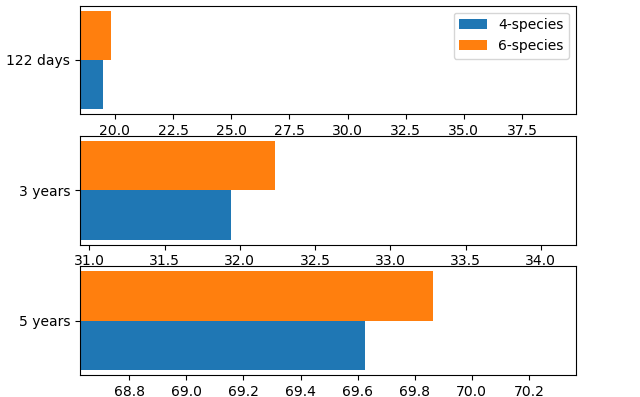
\includegraphics[width=\textwidth]{diversity.png}
    \end{minipage}
    \begin{minipage}{0.4\textwidth}
        \caption{The decomposition rate after a certain time of decay of 4-species and 6-species community. The two extra fungi species are weaker, meaning less competitive in pair wise test.}\label{fig:diversity}
    \end{minipage}
\end{figure}

Prediction as shown in figure \ref{fig:diversity} suggests that, when relatively weaker species are added into the community, the resulting decomposition efficiency is increased at a certain rate. Such effect becomes more significant when the experiment period extends longer. This result indicate that, biodiversity among the fungi community is positively related to the overall efficiency of a system with respect to the breakdown of ground litter.


\subsection{Sensitivity Analysis}

In our first model expressed \eqref{eq:decay-ability}, for the relation between decay ability and hyphal extension rate and moisture tolerance, with one-at-a-time method, presented great robustness. The environmental effect model is also robust against the varying of parameters or fungi properties. However, other parts of our work, especially Markov chain model and adaptive LV model are described implicitly through transition matrix or differential equations group, their robustness remains unknown unless tested massively through statistical measures.


\subsection{Strengths and Weaknesses}

The strengths and weaknesses of our model are both evident. For the strengths, our model

\begin{itemize}
    \item Extended the Lotka-Volterra model to multi-species cases, proposed the corresponding mathematical description. LV-model plays a significant role in ecological competition, but there not enough researches covering the multi-species condition. More the this, we also derived an adaptive form of LV model for fungi community based on the configuration of this problem.
    \item Implemented the notion of Markov chain process, to describe the homeostasis of the fungi community. The implementation of a discrete time, discrete status space model in a continuous problem is a bold attempt. Such concept offers brevity and convenience of calculation in our model.
    \item Incorporate the varying range of moisture as the affecting environmental factor, consider the fungi community as entirety, which also keeps consistent with the assumption that only the moisture niche width is taking effect.
    \item Also, in many other cases, the community is considered as an entirety, which provides remarkable integrity, convenience and consistency.
\end{itemize}

As for the weaknesses, our model

\begin{itemize}
    \item Ignored other detailed traits of fungi such as optimal moisture and temperature, some of them plays relatively important role in certain cases.
    \item Utilized implicit mathematical language to describe models, hence symbolical solutions cannot be found, and the intrinsic working principle remains uncertain.
    \item Took some assumptions that are less convincing and might even be incorrect.
\end{itemize}
